% Introduction chapter.
%%%%%%%%%%%%%%%%%%%%%%%

\chapter{Introduction}

The program relax is designed for the study of molecular dynamics through the analysis of experimental NMR data.
Organic molecules, proteins, RNA, DNA, sugars, and other biomolecules are all supported.
It was originally written for the model-free analysis of protein dynamics, though its scope has been significantly expanded.
It is a community driven project created by NMR spectroscopists for NMR spectroscopists.
It supports many analysis types including:

\begin{description}
\item[Model-free analysis] - the Lipari and Szabo model-free analysis of NMR relaxation data
\item[$\Rone$ and $\Rtwo$] - the exponential curve fitting for the calculation of the R$_x$ NMR relaxation rates.
\item[NOE] - the calculation of the steady-state NOE NMR relaxation data.
\item[Data consistency] - the consistency testing of multiple field NMR relaxation data.
\item[RSDM] - Reduced Spectral Density Mapping.
\item[Frame order and N-state model] - study of domain motions via the N-state model and frame order dynamics theories using anisotropic NMR parameters such as RDCs and PCSs.
\item[Stereochemistry] - investigations of absolute stereochemistry of flexible molecules.
\item[Relaxation dispersion] - the study of processes on the chemical exchange timescale.
\end{description}

The aim of relax is to provide a seamless and extremely flexible environment able to accept input in any format produced by other NMR software, able to faultlessly create input files, control, and read output from various programs including Modelfree and Dasha, output results in many formats, and visualise the data by controlling programs such as Grace\index{software!Grace|textbf}, OpenDX\index{software!OpenDX|textbf}, MOLMOL\index{software!MOLMOL|textbf}, and PyMOL\index{software!PyMOL|textbf}.
All data analysis tools from optimisation to model selection to Monte Carlo simulations are inbuilt into relax.
Therefore the use of additional programs is optional.

The flexibility of relax arises from the choice of relax's scripting capabilities, its Python\index{Python|textbf} prompt interface, or its graphical user interface (GUI)\index{User interface!GUI|textbf}.
Extremely complex scripts can be created from simple building blocks to fully automate data analysis.
A number of sample scripts have been provided to help understand script construction.
In addition, any of Python's powerful features or functions can be incorporated as the script is executed as an arbitrary Python source file within relax's environment.
The modules of relax can also used as a vast library of dynamics related functions by your own software.

relax is free software (free as in freedom) which is licenced under the GNU General Public Licence (GPL)\index{GPL|textbf}.
You are free to copy, modify, or redistribute relax under the terms of the GPL.


% Program features.
%%%%%%%%%%%%%%%%%%%

\section{Program features}


% Literature.
%~~~~~~~~~~~~

\subsection{Literature}

The primary references for the program relax are \citet{dAuvergneGooley08a} and \citet{dAuvergneGooley08b}.
To properly cite the various parts of relax used in your analysis, please see Chapter~\ref{ch: citations} on page~\pageref{ch: citations}.


% Supported NMR theories.
%~~~~~~~~~~~~~~~~~~~~~~~~

\subsection{Supported NMR theories}

The following relaxation data analysis techniques are currently supported by relax:

\begin{itemize}
\item Model-free analysis (\citet{LipariSzabo82a, LipariSzabo82b, Clore90a} and the specific implementation of \citet{dAuvergneGooley03,dAuvergneGooley06,dAuvergneGooley07,dAuvergneGooley08a,dAuvergneGooley08b}).
This includes the hybridisation of global diffusion models to study residual domain dynamics \citep{Horne07}.
\item Reduced spectral density mapping \citep{Farrow95, Lefevre96}\index{reduced spectral density mapping}.
\item Consistency testing -- the validation of multiple field NMR relaxation data \citep{MorinGagne09a,Fushman99}.
\item Exponential curve fitting (to find the $\Rone$ and $\Rtwo$ relaxation rates)\index{exponential curve fitting}.
\item Steady-state NOE calculation\index{NOE}.
\item Determination of absolute stereochemistry of flexible molecules via the N-state model using isotropic and anisotropic NMR parameters such as NOE, ROE, and RDC combined with MD simulation or simulated annealing, and ORD \citep{Sun11}.
\item The N-state model for investigating domain motions.
\item The frame order theory.
\item Conformational analysis of paramagnetically tagged molecules via the N-state model \citep{Erdelyi11}.
\item Analysis and comparison of ensembles of structures using RDCs, PCSs, NOEs, etc. (the N-state model of dynamics).
\item The analysis of relaxation dispersion\index{relaxation dispersion}.
\end{itemize}


% The future.
\subsubsection{The future}

Because relax is free software, if you would like to contribute addition features, functions, or modules which you have written for your own publications for the benefit of the field, almost anything relating to molecular dynamics may be accepted.
Please see the Open Source chapter on page~\pageref{ch: open source} for more details.



% Data analysis tools.
%~~~~~~~~~~~~~~~~~~~~~

\subsection{Data analysis tools}

The following tools are implemented as modular components to be used by any data analysis technique:

\begin{itemize}
\item Numerous high-precision optimisation algorithms\index{optimisation!algorithm}.
\item Model selection \citep{dAuvergneGooley03, Chen04}\index{model selection}:
    \begin{itemize}
    \item Akaike's Information Criteria (AIC)\index{model selection!AIC}.
    \item Small sample size corrected AIC (AICc)\index{model selection!AICc}.
    \item Bayesian or Schwarz Information Criteria (BIC)\index{model selection!BIC}.
    \item Bootstrap model selection\index{model selection!bootstrap}.
    \item Single-item-out cross-validation (CV)\index{model selection!cross-validation}.
    \item Hypothesis testing ANOVA model selection (only the model-free specific technique of \citet{Mandel95} is supported)\index{model selection!hypothesis testing}\index{model selection!ANOVA}.
    \end{itemize}
\item Monte Carlo simulations (error analysis for all data analysis techniques)\index{Monte Carlo simulation}.
\item Model elimination -- the removal of failed models prior to model selection \citep{dAuvergneGooley06}\index{model elimination}.
\end{itemize}


% Data visualisation.
%~~~~~~~~~~~~~~~~~~~~

\subsection{Data visualisation}

The results of an analysis, or any data input into relax, can be visualised using a number of programs:

\begin{description}
\item[MOLMOL] 1D data can be mapped onto a structure either by the creation of MOLMOL macros or by direct control of the program\index{software!MOLMOL}.
\item[PyMOL] 3D objects such as the diffusion tensor representation can be displayed with the structure\index{software!PyMOL}.
\item[Grace] any 2D data can be plotted\index{software!Grace}.
\item[OpenDX] The chi-squared space of models with three parameters can be mapped and 3D images of the space produced\index{software!OpenDX}.
\end{description}


% Interfacing with other programs.
%~~~~~~~~~~~~~~~~~~~~~~~~~~~~~~~~~

\subsection{Interfacing with other programs}

relax can create the input files, execute in-line, and then read the output of the following programs.
These programs can be used as optimisation engines replacing the minimisation algorithms built into relax:

\begin{itemize}
\item Dasha (model-free analysis)\index{software!Dasha}.
\item Modelfree (model-free analysis)\index{software!Modelfree}.
\end{itemize}


% The user interfaces (UI).
%~~~~~~~~~~~~~~~~~~~~~~~~~~

\subsection{The user interfaces (UI)}

relax can be used through the following UIs:

\begin{description}
\item[The prompt] this is the primary interface of relax.
Rather than reinventing a new command language, relax's interface is the powerful Python prompt.
This gives the power user full access to a proven programming language.
See Figure~\ref{fig: relax prompt} for a screenshot.
\item[Scripting] this provides a more powerful and flexible framework for controlling the program.
The script will be executed as Python code enabling advanced programming for automating data analysis.
All the features available within the prompt environment are accessible to the script.
See Figure~\ref{fig: relax script} for a screenshot.
\item[GUI] the graphical user interface provides a sub-set of relax's features - the automatic R$_1$ and R$_2$ relaxation rate curve-fitting, the NOE calculations, and the automatic model-free analysis provided by the \module{dauvergne\pyus{}protocol} module \citep{dAuvergneGooley08b}.
See Figure~\ref{fig: GUI screenshot - start} for a screenshot.
\end{description}



% The relax HOWTO.
%%%%%%%%%%%%%%%%%%

\section{How to use relax}


% The prompt.
%~~~~~~~~~~~~

\subsection{The prompt}
\index{User interface!prompt|textbf}

The primary interface of relax is the prompt.
After typing \promptstring{relax} within a terminal\index{terminal} you will be presented with

\begin{lstlisting}[numbers=none]
relax>
\end{lstlisting}

This is the Python prompt which has been tailored specifically for relax.
You will hence have full access, if desired, to the power of the Python\index{Python} programming language to manipulate your data.
You can for instance type

\begin{lstlisting}[numbers=none]
relax> print("Hello World")
\end{lstlisting}

the result being

\begin{lstlisting}[numbers=none]
relax> print("Hello World")
Hello World
relax>
\end{lstlisting}

Or using relax as a calculator

\begin{lstlisting}[numbers=none]
relax> (1.0 + (2 * 3))/10
0.69999999999999996
relax>
\end{lstlisting}

% Prompt screenshot
\begin{figure}
\centerline{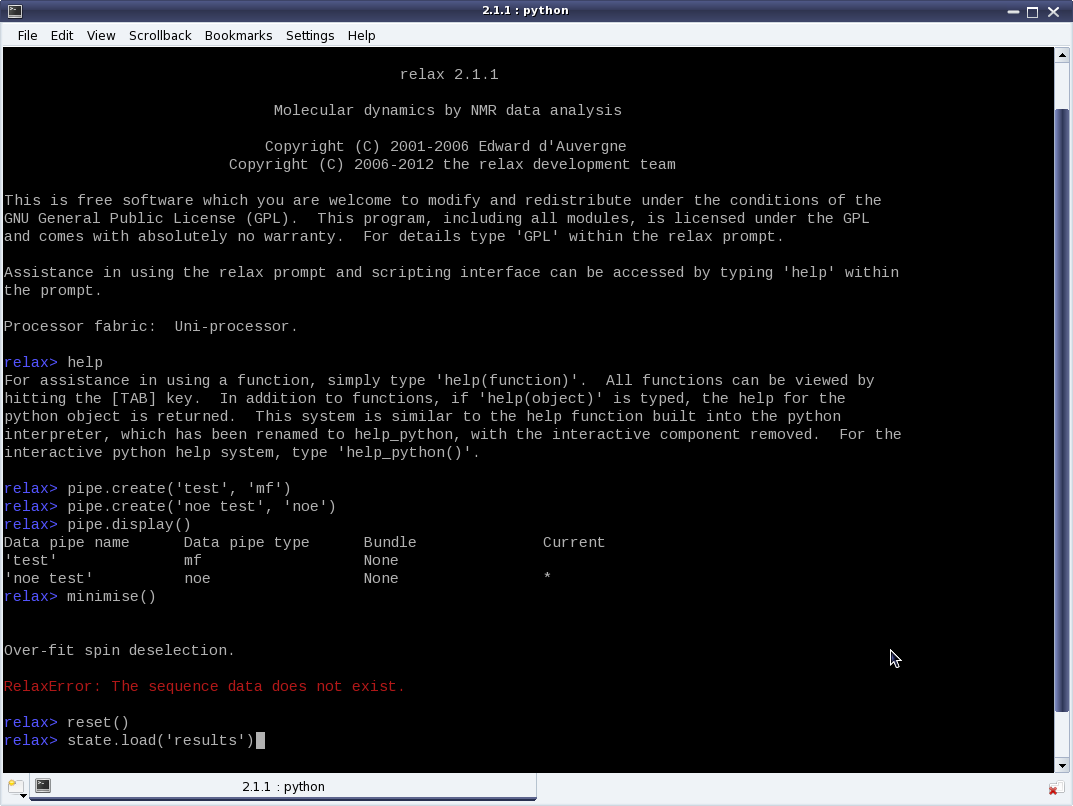
\includegraphics[width=0.9\textwidth, bb=14 14 1088 821]{graphics/screenshots/relax_prompt_mode}}
\caption[Prompt screenshot]{A screenshot of relax being run in the primary prompt mode.}\label{fig: relax prompt}
\end{figure}



% Python.
%~~~~~~~~

\subsection{Python}

\index{Python|textbf}
relax has been designed such that knowledge about Python is not required to be able to fully use the program.
A few basics though will aid in understanding relax.

A number of simple programming axioms includes that of strings\index{string}, integers\index{integer}, floating point numbers\index{floating point number}, and lists\index{list}.
A string is text and within Python (as well as relax) this is delimited by either single or double quotes.
An integer is a number with no decimal point whereas a float is a number with a decimal point.
A list in Python (called an array in other languages) is a list of anything separated by commas and delimited by square brackets, an example is \prompt{[0, 1, 2, `a', 1.2143235]}.

Probably the most important detail is that functions in Python require brackets around their arguments.
For example

\begin{lstlisting}[numbers=none]
relax> minimise()
\end{lstlisting}

will commence minimisation\index{optimisation} however

\begin{lstlisting}[numbers=none]
relax> minimise
\end{lstlisting}

will do nothing.

The arguments to a function are simply a comma separated list within the brackets of the function.
For example to save the program's current state type

\begin{lstlisting}[numbers=none]
relax> state.save('save', force=True)
\end{lstlisting}

Two types of arguments exist in Python\index{Python|textbf} -- standard arguments\index{argument} and keyword arguments\index{argument!keyword}.
The majority of arguments you will encounter within relax are keyword arguments however you may, in rare cases, encounter a non-keyword argument.
For these standard arguments just type the values in, although they must be in the correct order.
Keyword arguments consist of two parts -- the key and the value.
For example the key may be \prompt{file} and the value you would like to supply is \promptstring{R1.out}.
Various methods exist for supplying this argument.
Firstly you could simply type \promptstring{R1.out} into the correct position in the argument list.
Secondly you can type \prompt{file=`R1.out'}.
The power of this second option is that argument order is unimportant.
Therefore if you would like to change the default value of the very last argument, you don't have to supply values for all other arguments.
The only catch is that standard arguments must come before the keyword arguments.


% Script screenshot
\begin{figure}
\centerline{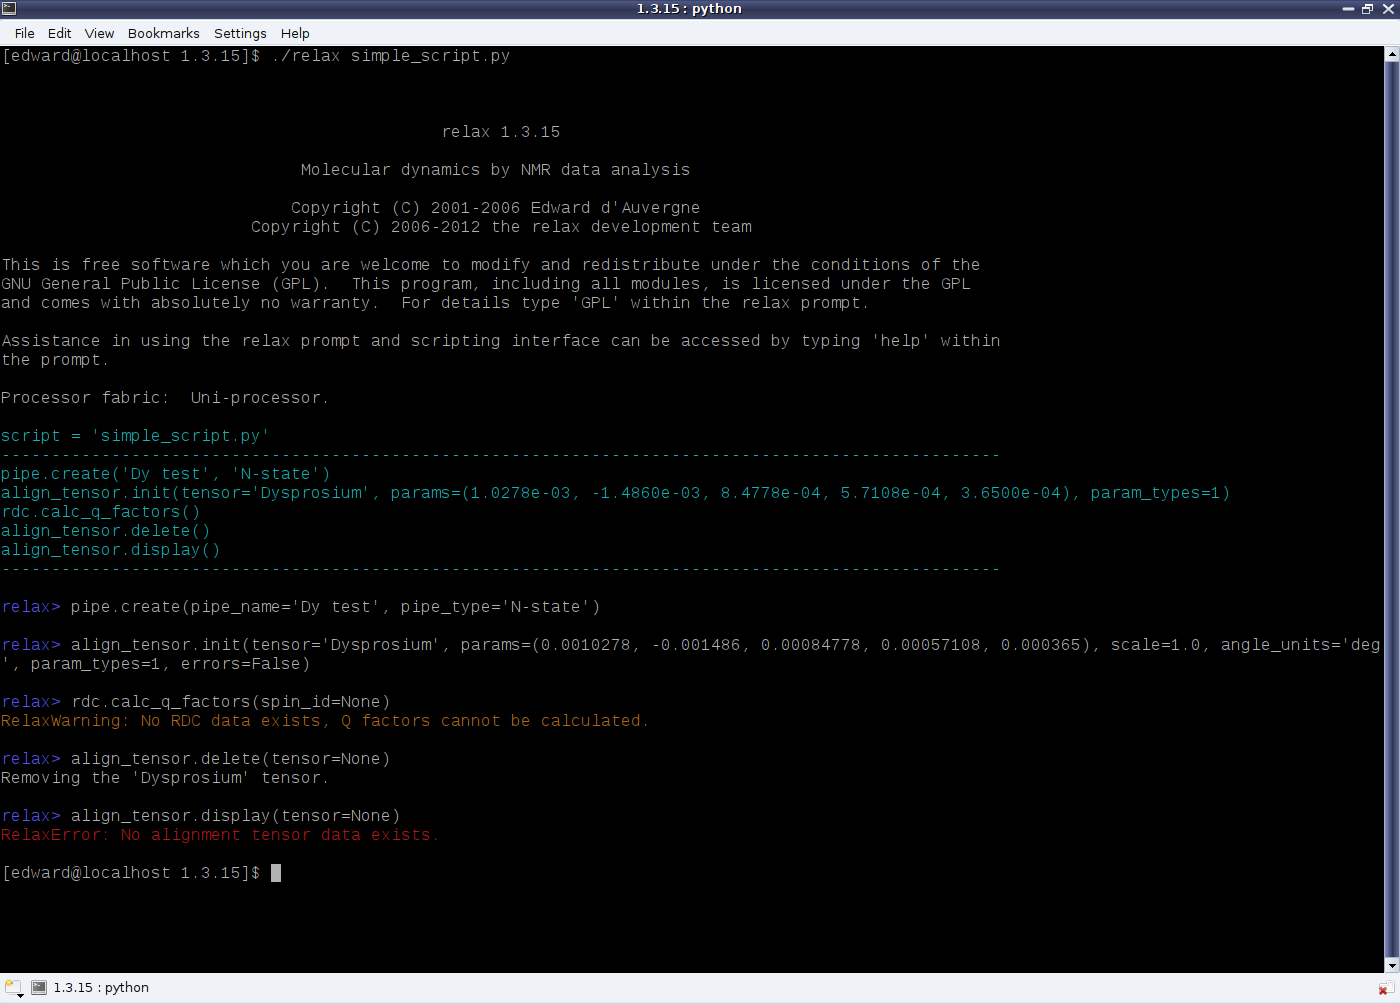
\includegraphics[width=0.9\textwidth, bb=14 14 1065 768]{graphics/screenshots/relax_script_mode}}
\caption[Scripting screenshot]{A screenshot of relax being run in scripting mode.}\label{fig: relax script}
\end{figure}


% User functions.
%~~~~~~~~~~~~~~~~

\subsection{User functions}
\index{user functions|textbf}

For standard data analysis a large number of specially tailored functions called ``user functions'' have been implemented.
These are accessible from the relax prompt by simply typing the name of the function.
An example is \uf{help()}\index{help system}.
An alphabetical listing of all accessible user functions together with full descriptions is presented later in this manual.

A few special objects which are available within the prompt are not actually functions.
These objects do not require brackets at their end for them to function.
For example to exit relax type

\begin{lstlisting}[numbers=none]
relax> exit
\end{lstlisting}

Another special object is that of the function class\index{function class}.
This object is simply a container which holds a number of user functions.
You can access the user function within the class by typing the name of the class, then a dot \promptstring{.}, followed by the name of the user function.
An example is the user function for reading relaxation data out of a file and loading the data into relax.
The function is called \promptstring{read} and the class is called \promptstring{relax\_data}.
To execute the function, type something like

\begin{lstlisting}[numbers=none]
relax> relax_data.read(ri_id='R1_600',  ri_type='R1',  frq=600.0*1e6, file='r1.600.out', res_num_col=1, data_col=3, error_col=4)
\end{lstlisting}

On first usage the relax prompt can be quite daunting.
Two features exist to increase the usability of the prompt -- the help system and tab completion.



% The help system.
%~~~~~~~~~~~~~~~~~

\subsection{The help system}
\index{help system|textbf}

For assistance in using a function simply type

\begin{lstlisting}[numbers=none]
relax> help(function)
\end{lstlisting}

In addition to functions if

\begin{lstlisting}[numbers=none]
relax> help(object)
\end{lstlisting}

is typed the help for the python object is returned.
This system is similar to the help function built into the python interpreter, which has been renamed to \prompt{help\_python}, with the interactive component removed.
For the standard interactive python help system type

\begin{lstlisting}[numbers=none]
relax> help_python()
\end{lstlisting}




% Tab completion.
%~~~~~~~~~~~~~~~~

\subsection{Tab completion}
\index{tab completion|textbf}

Tab completion is implemented to prevent insanity as the function names can be quite long -- a deliberate feature to improve usability.
The behaviour of the tab completion is very similar to that of the bash prompt.

Not only is tab completion useful for preventing RSI but it can also be used for listing all available functions.
To begin with if you hit the [TAB] key without typing any text all available functions will be listed (along with function classes\index{function class} and other python objects).
This extends to the exploration of user functions\index{user functions} within a function class\index{function class}.
For example to list the user functions within the function class \uf{model\ufus{}free} type

\begin{lstlisting}[numbers=none]
relax> model_free.
\end{lstlisting}

The dot character at the end is essential.
After hitting the [TAB] key you should see something like

\begin{lstlisting}[numbers=none]
relax| model_free.
model_free.__class__
model_free.__doc__
model_free.__init__
model_free.__module__
model_free.__relax__
model_free.__relax_help__
model_free.create_model
model_free.delete
model_free.remove_tm
model_free.select_model
relax> model_free.
\end{lstlisting}

All the objects beginning with an underscore are ``hidden'', they contain information about the function class\index{function class} and should be ignored.
From the listing the user functions\index{user functions} \uf{copy}, \uf{create\ufus{}model}, \uf{delete}, \uf{remove\ufus{}tm}, and \uf{select\ufus{}model} contained within \uf{model\ufus{}free} are all visible.

% GUI screenshot
\begin{figure}
\centerline{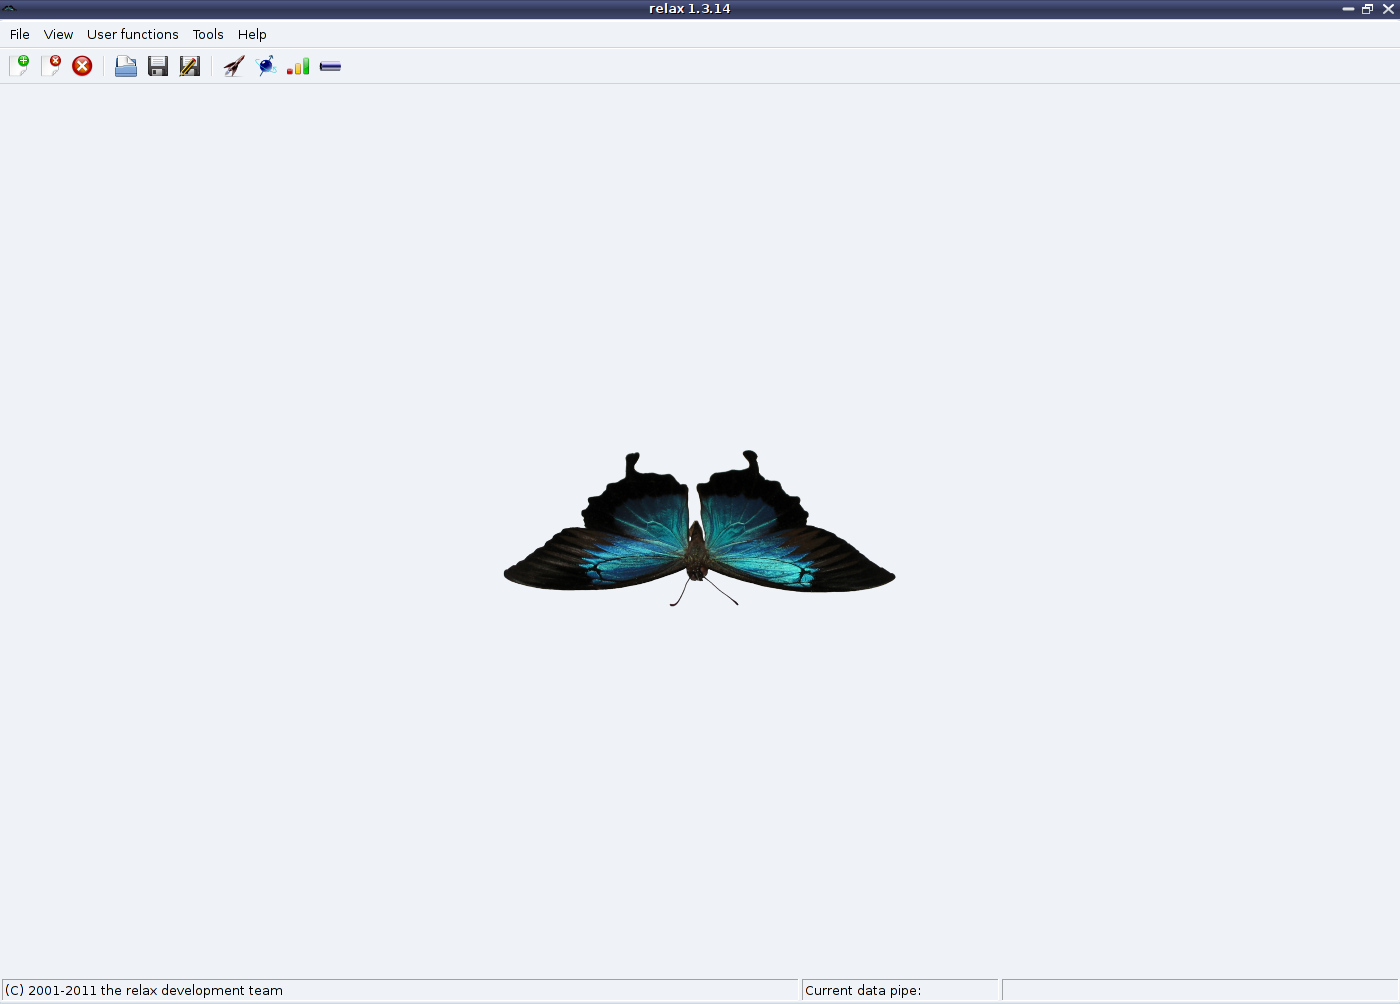
\includegraphics[width=0.9\textwidth, bb=14 14 1065 768]{graphics/screenshots/start}}
\caption[GUI screenshot]{Screenshot of the relax GUI interface -- the starting interface.  To start one of the automated analyses, either the menu \guimenuitemtwo{File}{New analysis} or the new analysis button in the toolbar should be selected.}\label{fig: GUI screenshot - start}
\end{figure}



% The data pipe.
%~~~~~~~~~~~~~~~

\subsection{The data pipe} \label{sect: the data pipe}
\index{data pipe|textbf}

Within relax all user functions operate on data stored within the current data pipe.
This pipe stores data is input, processed, or output as user functions are called.
There are different types of data pipe for different analyses, e.g. a reduced spectral density mapping pipe, a model-free pipe, an exponential curve-fitting pipe, etc.
Multiple data pipes can be created within relax and various operations performed in sequence on these pipes.
This is useful for operations such as model selection whereby the function \uf{model\ufus{}selection} can operate on a number of pipes corresponding to different models and then assign the results to a newly created pipe.
When running relax you choose which pipe you are currently in by using the \uf{pipe\ufsep{}switch} user function to jump between pipes.

The flow of data through relax can be thought of as travelling through these pipes.
User functions\index{user functions} exist to transfer data between these pipes and other functions combine data from multiple pipes into one or vice versa.
The simplest invocation of relax would be the creation of a single data pipe and with the data being processed as it is passing through this pipe.

The primary method for creating a data pipe is through the user function\index{user functions} \uf{pipe\ufsep{}create}.
For example

\begin{lstlisting}[numbers=none]
relax> pipe.create('m1', 'mf')
\end{lstlisting}

will create a model-free data pipe labelled \promptstring{m1}.
The following is a table of all the types which can be assigned to a data pipe.

\begin{center}
\begin{tabular}{ll}
\toprule

Data pipe type          & Description \\

\midrule

\promptstring{ct}           & Consistency testing of relaxation data \\
\promptstring{frame order}  & The Frame Order analyses of domain motions \\
\promptstring{jw}           & Reduced spectral density mapping \\
\promptstring{hybrid}       & A special hybridised data pipe \\
\promptstring{mf}           & Model-free data analysis \\
\promptstring{N-state}      & N-state model of domain motions \\
\promptstring{noe}          & Steady state NOE calculation \\
\promptstring{relax\_fit}   & Relaxation curve-fitting \\

\bottomrule
\end{tabular}
\end{center}



% The spin and interatomic data containers.
%~~~~~~~~~~~~~~~~~~~~~~~~~~~~~~~~~~~~~~~~~~

\subsection{The spin and interatomic data containers}
\index{spin container|textbf}
\index{interatomic data container|textbf}

Any data which is not considered global for the molecule, such as diffusion tensors, alignment tensors, global minimisation statistics, etc., are stored within two special structures of the data pipes.
Any NMR data or information which is specific to an isolated spin system is stored within special spin containers.
This includes for example relaxation data, CSA information, nuclear isotope type, chemical element type, model-free parameters, reduced spectral density mapping values, spin specific minimisation statistics and PCS data.
NMR data or information which is defined as being between two spin systems, such as the magnetic dipole-dipole interaction involved in both NMR relaxation and RDC data, interatomic vectors and NOESY data, is stored within the interatomic data containers.
The spin and interatomic data containers and their associated data can be manipulated using a multitude of the relax user functions.


% Analysis wizard screenshot
\begin{figure}
\centerline{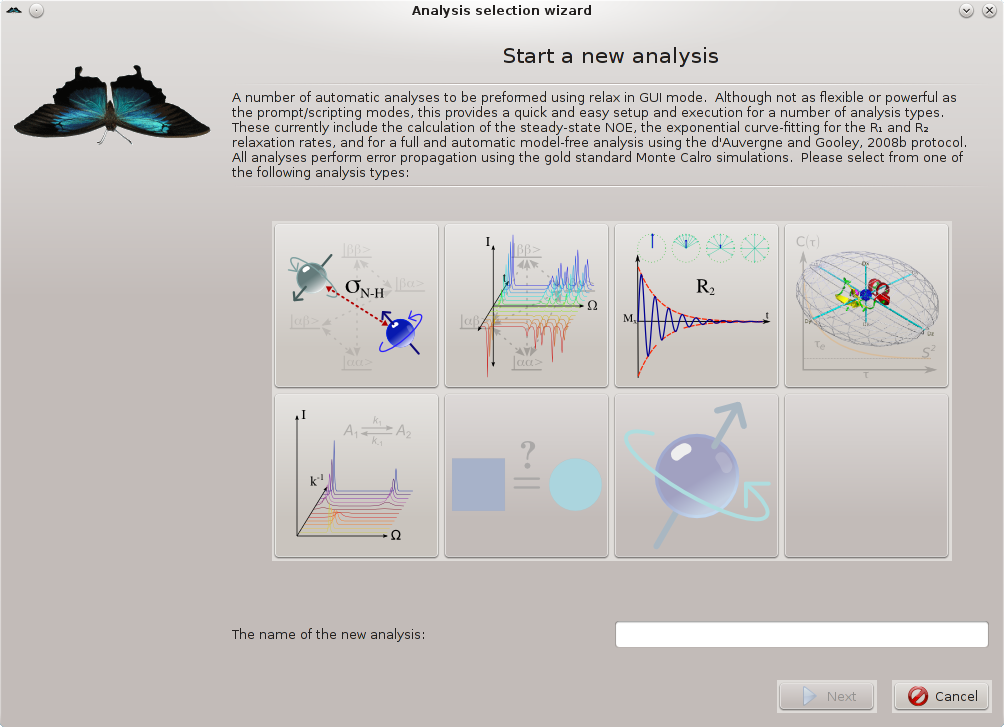
\includegraphics[width=0.8\textwidth, bb=14 14 768 560]{graphics/screenshots/analysis_wizard}}
\caption[GUI screenshot -- Analysis wizard screenshot]{Screenshot of the relax GUI interface -- the analysis selection wizard.  From here, the steady-state NOE analysis, the $\Rone$ and $\Rtwo$ relaxation rates via exponential curve-fitting, and the automated model-free analysis can be selected.}\label{fig: screenshot: analysis wizard}
\end{figure}



% Scripting.
%~~~~~~~~~~~

\subsection{Scripting} \label{sect: scripting}
\index{User interface!scripting|textbf}

What ever is done within the prompt is also accessible through scripting (Figure~\ref{fig: relax script}).
First type your commands into a text file ending in \file{*.py}.
To use this mode of relax, you will need to open up a terminal in your respective operating system:

\begin{description}
\item[GNU/Linux:]  Here you have an incredible number of choices.
If you don't have a preferred shell already, you could try one of \software{Konsole}, \software{GNOME Terminal} or even \software{XTerm} if you are a masochist.
\item[Mac OS X:]  This is as simple as in GNU/Linux -- just launch \software{Terminal.app} from the \directory{Utilities} folder.
\item[MS Windows:]  If your system supports it, you should install and use \software{Windows PowerShell}.
The alternative is the nasty \software{cmd} command line terminal program which comes installed by default on all Windows versions.
The \software{PowerShell}, although no where near as powerful as the Linux and Mac terminals, is a huge improvement on the ancient \software{cmd} program and will make relax much better to use on MS Windows.
\end{description}

Once your terminal is running, go to the directory containing your script using the \prompt{cd} command (if you do not know what this is, please see the documentation for your terminal program to understand some of its basic usage).
Once you are in the correct directory, within the terminal type:

\example{\$ relax your\_script.py}

You will need to replace \file{your\osus{}script.py} with the name of your script.
In most cases you would probably like to keep a log of all of the messages, warnings and errors relax produces for future reference.
To active logging within relax, type:

\example{\$ relax --log log your\_script.py}

This will place all output (both STDOUT and STDERR) into the \file{log} file (you can choose any name for this log file).
Alternatively you can both log the output and simultaneously see the messages in your terminal by typing:

\example{\$ relax --tee log your\_script.py}

These command line arguments could be replaced by IO redirection if this is a familiar concept to you, but note that these arguments are active also in the GUI mode whereby IO redirection in the terminal will have no effect.
An example of a simple script which will minimise the model-free model ``m4'' after loading six relaxation data sets is

\begin{lstlisting}
# Create the data pipe.
name = 'm4'
pipe.create(name, 'mf')

# Load the PDB file.
structure.read_pdb('1f3y.pdb')

# Set up the 15N and 1H spins.
structure.load_spins('@N', ave_pos=True)
structure.load_spins('@H', ave_pos=True)
spin.isotope('15N', spin_id='@N')
spin.isotope('1H', spin_id='@H')

# Load the relaxation data.
relax_data.read(ri_id='R1_600',  ri_type='R1',  frq=600.0*1e6, file='r1.600.out', res_num_col=1, data_col=3, error_col=4)
relax_data.read(ri_id='R2_600',  ri_type='R2',  frq=600.0*1e6, file='r2.600.out', res_num_col=1, data_col=3, error_col=4)
relax_data.read(ri_id='NOE_600', ri_type='NOE', frq=600.0*1e6, file='noe.600.out', res_num_col=1, data_col=3, error_col=4)
relax_data.read(ri_id='R1_500',  ri_type='R1',  frq=500.0*1e6, file='r1.500.out', res_num_col=1, data_col=3, error_col=4)
relax_data.read(ri_id='R2_500',  ri_type='R2',  frq=500.0*1e6, file='r2.500.out', res_num_col=1, data_col=3, error_col=4)
relax_data.read(ri_id='NOE_500', ri_type='NOE', frq=500.0*1e6, file='noe.500.out', res_num_col=1, data_col=3, error_col=4)

# Initialise the diffusion tensor.
diffusion_tensor.init((2e-8, 1.3, 60, 290), spheroid_type='prolate', param_types=2, fixed=True)

# Create all attached protons.
sequence.attach_protons()

# Define the magnetic dipole-dipole relaxation interaction.
interatom.define(spin_id1='@N', spin_id2='@H', direct_bond=True)
interatom.set_dist(spin_id1='@N', spin_id2='@H', ave_dist=1.02 * 1e-10)
interatom.unit_vectors()

# Define the CSA relaxation interaction.
value.set(-172 * 1e-6, 'csa')

# Select a preset model-free model.
model_free.select_model(model=name)

# Grid search.
grid_search(inc=11)

# Minimise.
minimise('newton')

# Finish.
results.write(file='results', force=True)
state.save('save', force=True)
\end{lstlisting}

Scripting is much more powerful than the prompt as advanced Python\index{Python} programming can be employed (see the file \file{relax\osus{}curve\osus{}diff.py} in the \directory{sample\osus{}scripts} directory for an example).



% Sample scripts.
\subsubsection{Sample scripts}
\index{scripting!sample scripts}

A few sample scripts have been provided in the directory \directory{sample\osus{}scripts}.
These can be copied and modified for different types of data analysis.



% The test suite.
%~~~~~~~~~~~~~~~~

\subsection{The test suite}
\index{test suite}

To test that the program functions correctly, relax possesses an inbuilt test suite.
The suite is a collection of simple tests which execute or probe different parts of the program checking that the software runs without problem.
The test suite is executed by running relax using the command

\example{\$ relax --test-suite}

Alternatively the three components of the test suite -- system tests, unit tests, and GUI tests -- can be run separately with

\example{\$ relax --system-tests}

\example{\$ relax --unit-tests}

\example{\$ relax --gui-tests}


% NOE analysis screenshot
\begin{figure}
\centerline{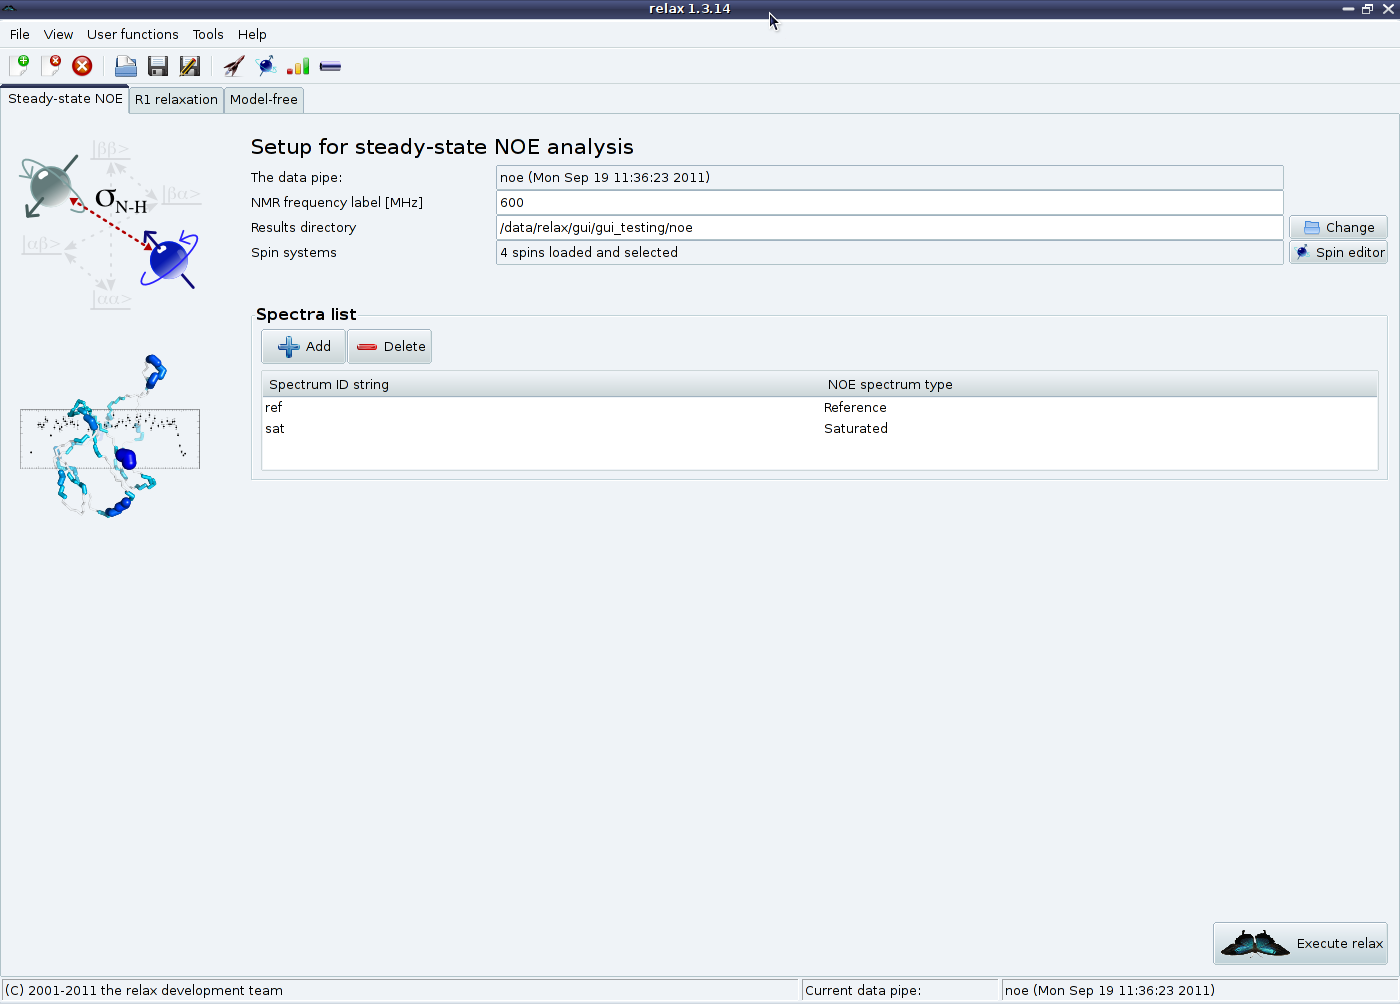
\includegraphics[width=\textwidth, bb=14 14 1065 768]{graphics/screenshots/analysis_noe}}
\caption[GUI screenshot -- NOE analysis]{Screenshot of the relax GUI interface -- the steady-state NOE analysis.}\label{fig: screenshot: NOE analysis}
\end{figure}


% The GUI.
%~~~~~~~~~

\subsection{The GUI}
\index{User interface!GUI|textbf}

% R1 analysis screenshot
\begin{figure}
\centerline{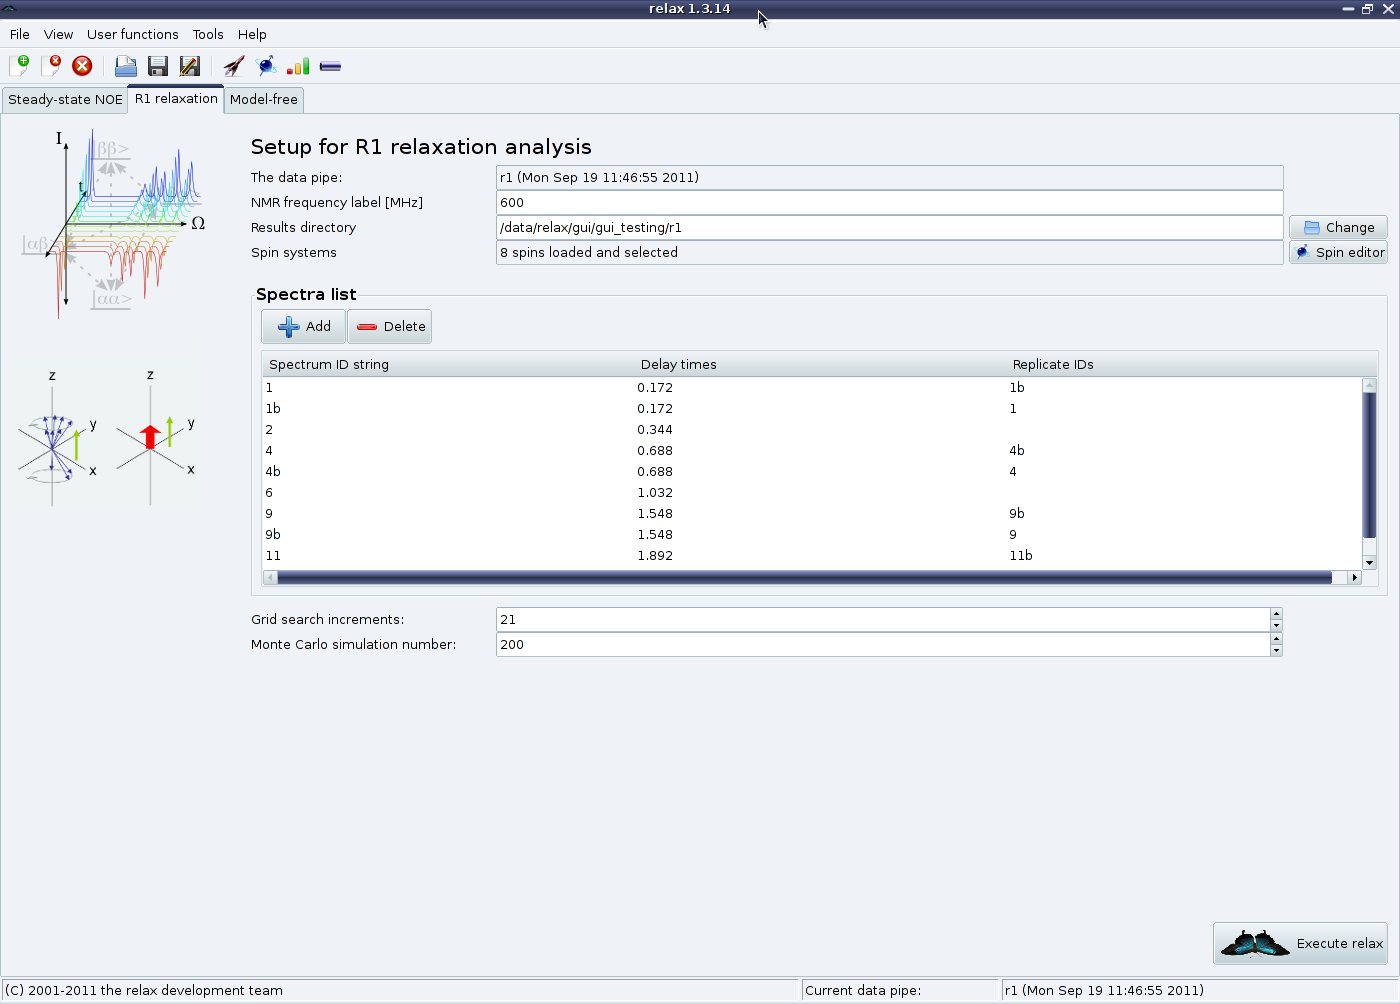
\includegraphics[width=\textwidth, bb=14 14 1065 768]{graphics/screenshots/analysis_r1}}
\caption[GUI screenshot -- $\Rone$ analysis]{Screenshot of the relax GUI interface -- the $\Rone$ analysis.}\label{fig: screenshot: R1 analysis}
\end{figure}


% R2 analysis screenshot
\begin{figure}
\centerline{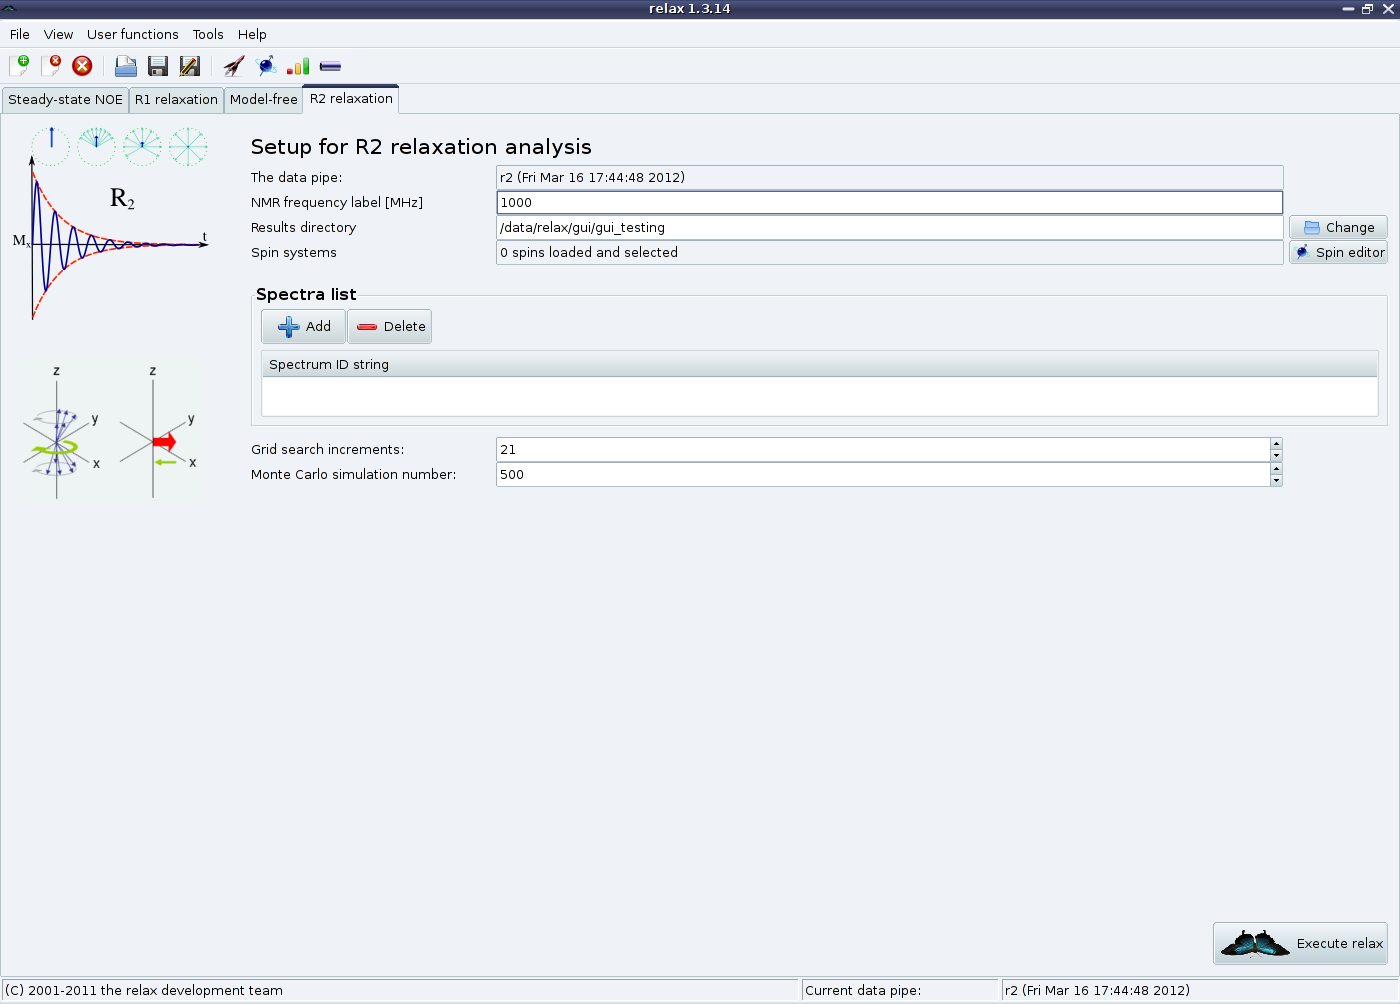
\includegraphics[width=\textwidth, bb=14 14 1065 768]{graphics/screenshots/analysis_r2}}
\caption[GUI screenshot -- $\Rtwo$ analysis]{Screenshot of the relax GUI interface -- the $\Rtwo$ analysis.}\label{fig: screenshot: R2 analysis}
\end{figure}

If the wxPython module is installed on your system, you will have access to the GUI interface of relax.
To launch relax in GUI mode, type either

\example{\$ relax -g}

or

\example{\$ relax --gui}

In most cases you will probably like to have a permanent copy of all the messages, warnings, and errors relax produces for future reference.
In such a case you could run the GUI with:

\example{\$ relax --gui --log log}

This will place all of the output into the \file{log} file.

% Model-free analysis screenshot
\begin{figure}
\centerline{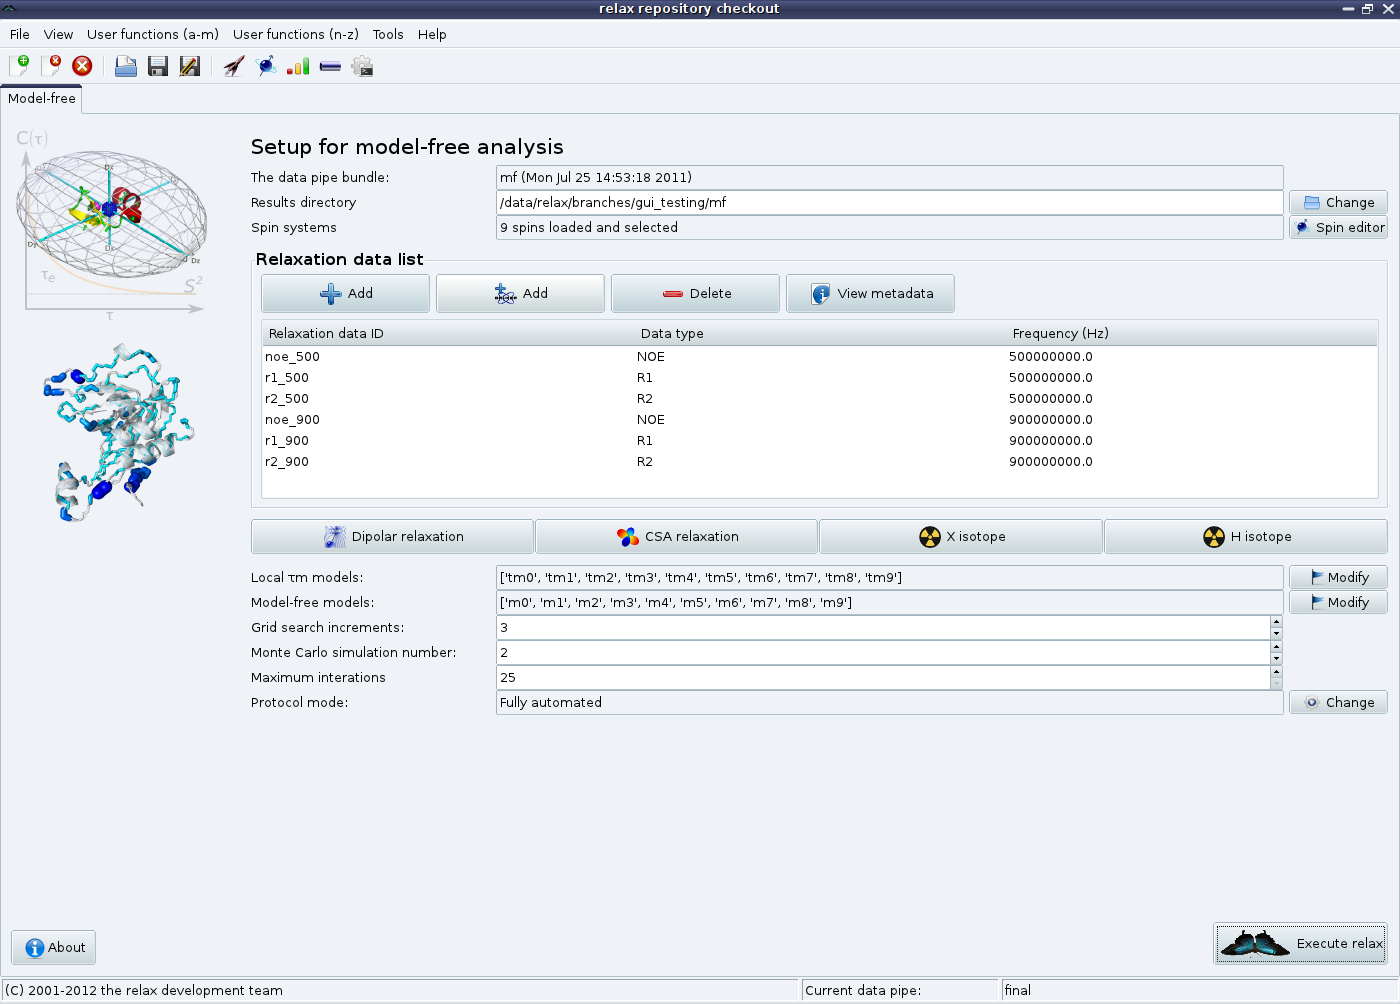
\includegraphics[width=\textwidth, bb=14 14 1065 768]{graphics/screenshots/analysis_mf}}
\caption[GUI screenshot -- Model-free analysis]{Screenshot of the relax GUI interface -- the automated model-free analysis.  The analysis is fully automated via a new model-free protocol as described in detail in Chapter~\ref{ch: model-free}.  Clicking on the \guibutton{About} button in the bottom left hand corner will give a full description of the protocol.  For using this interface or any of the modern-day model-free protocols, data from at least two magnetic field strengths must be without question collected.}\label{fig: screenshot: model-free analysis}
\end{figure}

The GUI is currently an interface to the automated analyses, providing an easy way to perform quick analyses.
The interface consists of a tab for each analysis.
By clicking on the \guimenuitemtwo{File}{New analysis} menu entry or the \guibutton{New analysis} toolbar button, the analysis wizard will appear (see Figure~\ref{fig: screenshot: analysis wizard}).
The following analyses can be set up using this wizard:

\begin{description}
\item[Steady-state NOE:]  this provides access to the steady-state NOE calculation with pseudo Monte Carlo simulations for error analysis (this falls back to bootstrapping as this is a calculation rather than optimisation).
See Figure~\ref{fig: screenshot: NOE analysis} on page~\pageref{fig: screenshot: NOE analysis}.
\item[$\Rone$ and $\Rtwo$]:  these provide easy access to optimisations and error analysis for the $\Rone$ and $\Rtwo$ relaxation rates via exponential curve-fitting (see Figures~\ref{fig: screenshot: R1 analysis} and~\ref{fig: screenshot: R2 analysis} on pages~\pageref{fig: screenshot: R1 analysis} and~\pageref{fig: screenshot: R2 analysis}).
\item[Model-free analysis]:  A fully automatic model-free protocol is provided in another tab.
This operates via the \module{dauvergne\pyus{}protocol} module which implements the protocol of \cite{dAuvergneGooley08b} (see Figure~\ref{fig: screenshot: model-free analysis} on page~\pageref{fig: screenshot: model-free analysis}).
\end{description}

A number of windows in the GUI provide user feedback or allow for the viewing and editing of data.
These include:

% relax controller screenshot
\begin{figure}
\centerline{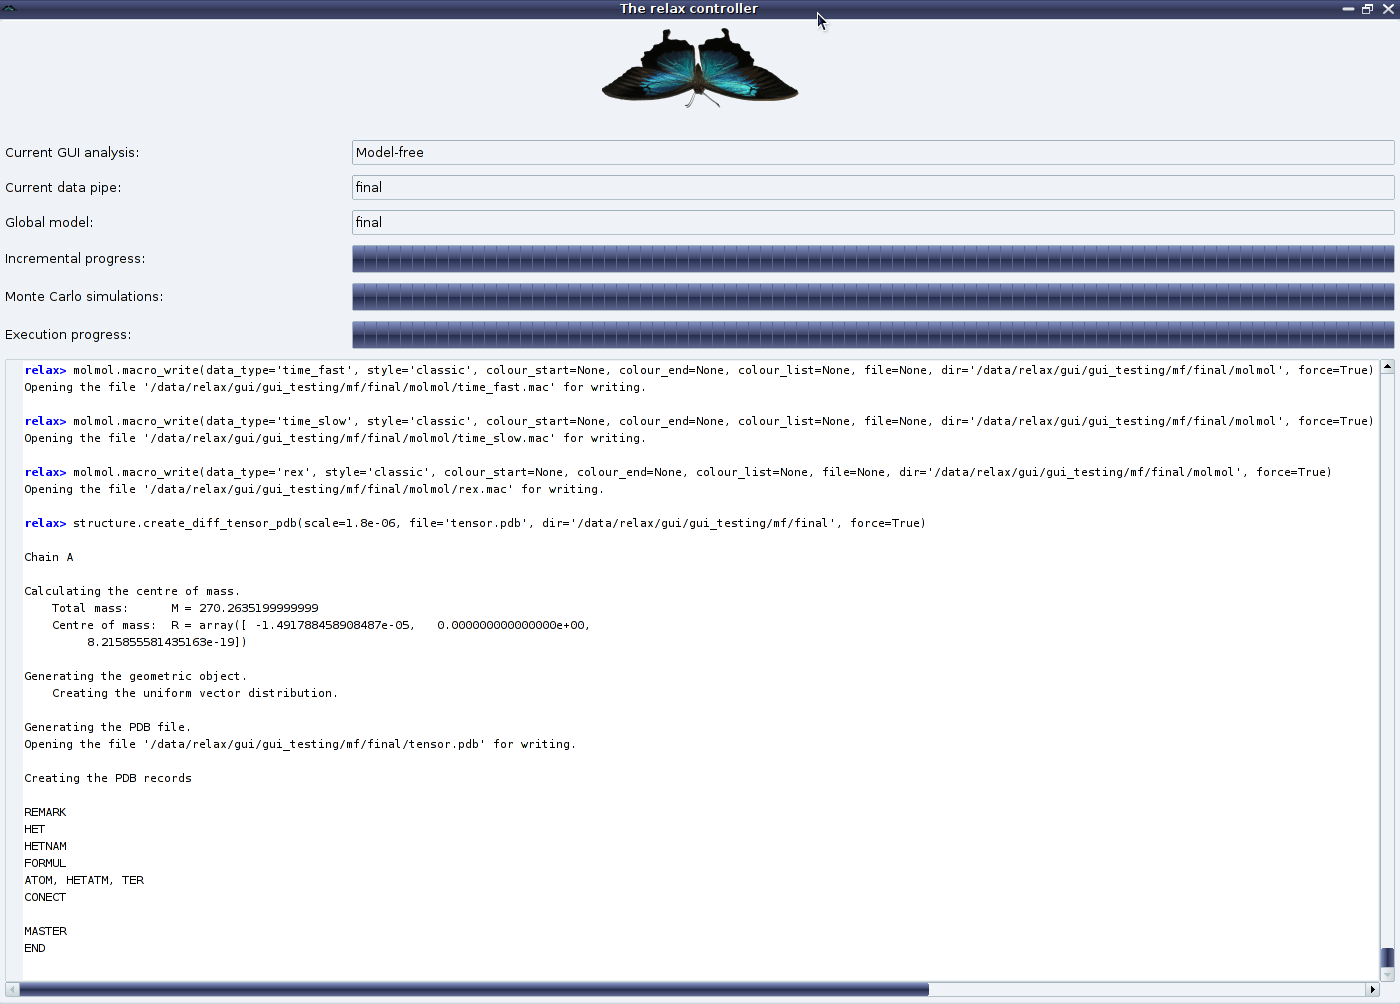
\includegraphics[width=0.9\textwidth, bb=14 14 1065 768]{graphics/screenshots/relax_controller}}
\caption[relax controller screenshot]{Screenshot of the relax GUI interface -- the relax controller window.  The purpose of the controller is for feedback.  It shows the current analysis and current data pipe, a number of progress gauges, and the relax text output.}\label{fig: screenshot: relax controller}
\end{figure}

% Spin viewer screenshot
\begin{figure}
\centerline{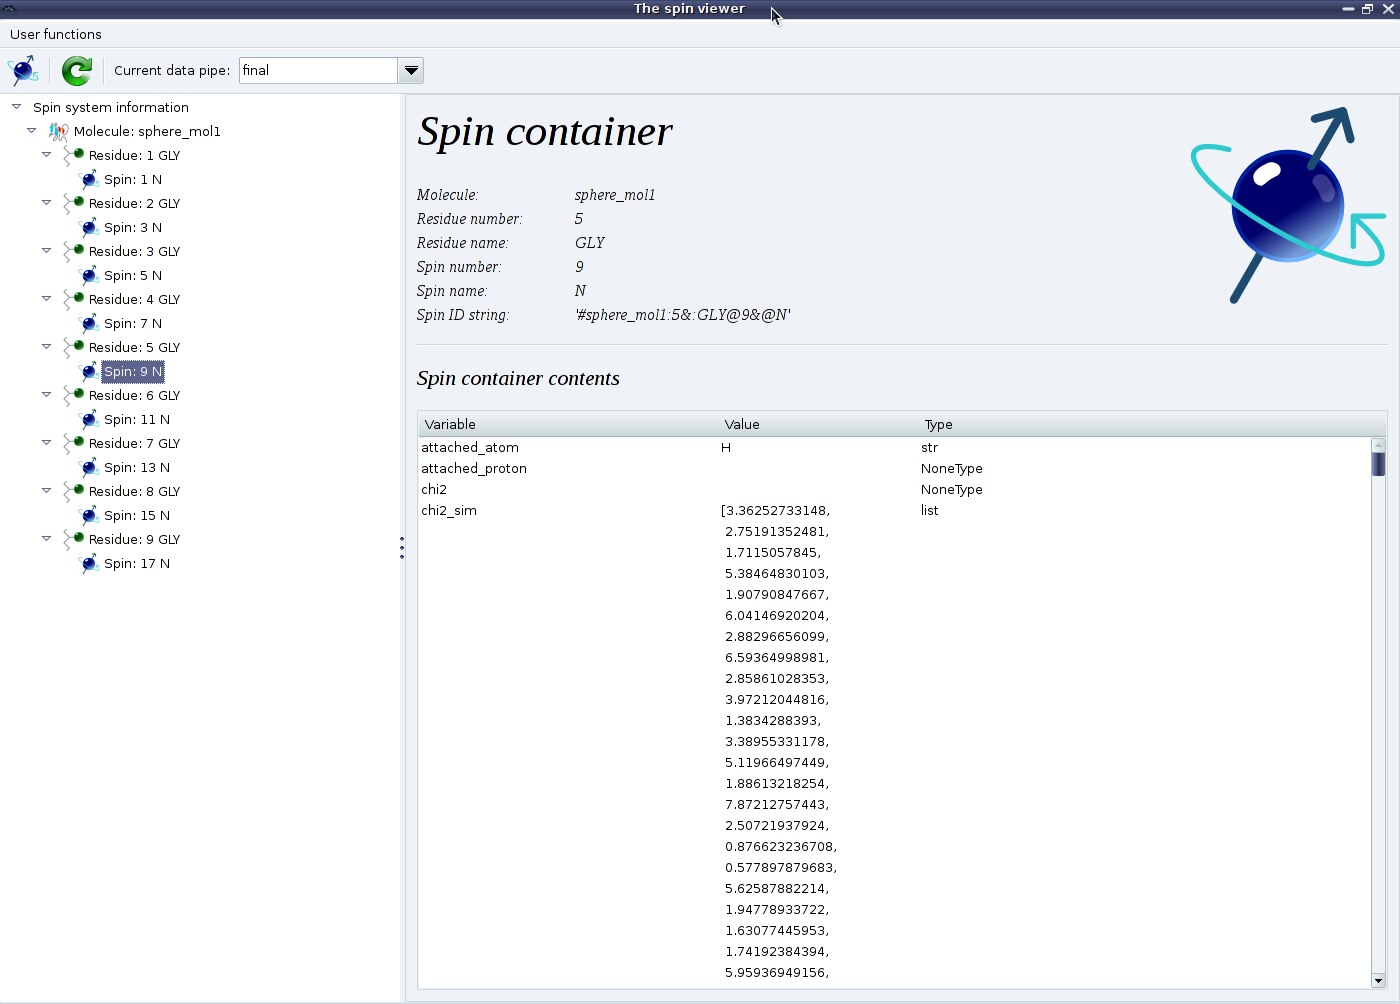
\includegraphics[width=0.9\textwidth, bb=14 14 1065 768]{graphics/screenshots/spin_viewer}}
\caption[Spin viewer window screenshot]{Screenshot of the relax GUI interface -- the spin viewer window.  This viewer is designed for easy addition and manipulation of spin systems within the relax data store.  The window is accessible via the \guimenuitemtwo{View}{Spin viewer} menu entry, typing \shortcutkey{Ctrl-T}, the spin viewer button in the toolbar, or the \guibutton{spin editor} button within the auto-analysis tabs.}\label{fig: screenshot: spin viewer}
\end{figure}

% Results viewer screenshot
\begin{figure}
\centerline{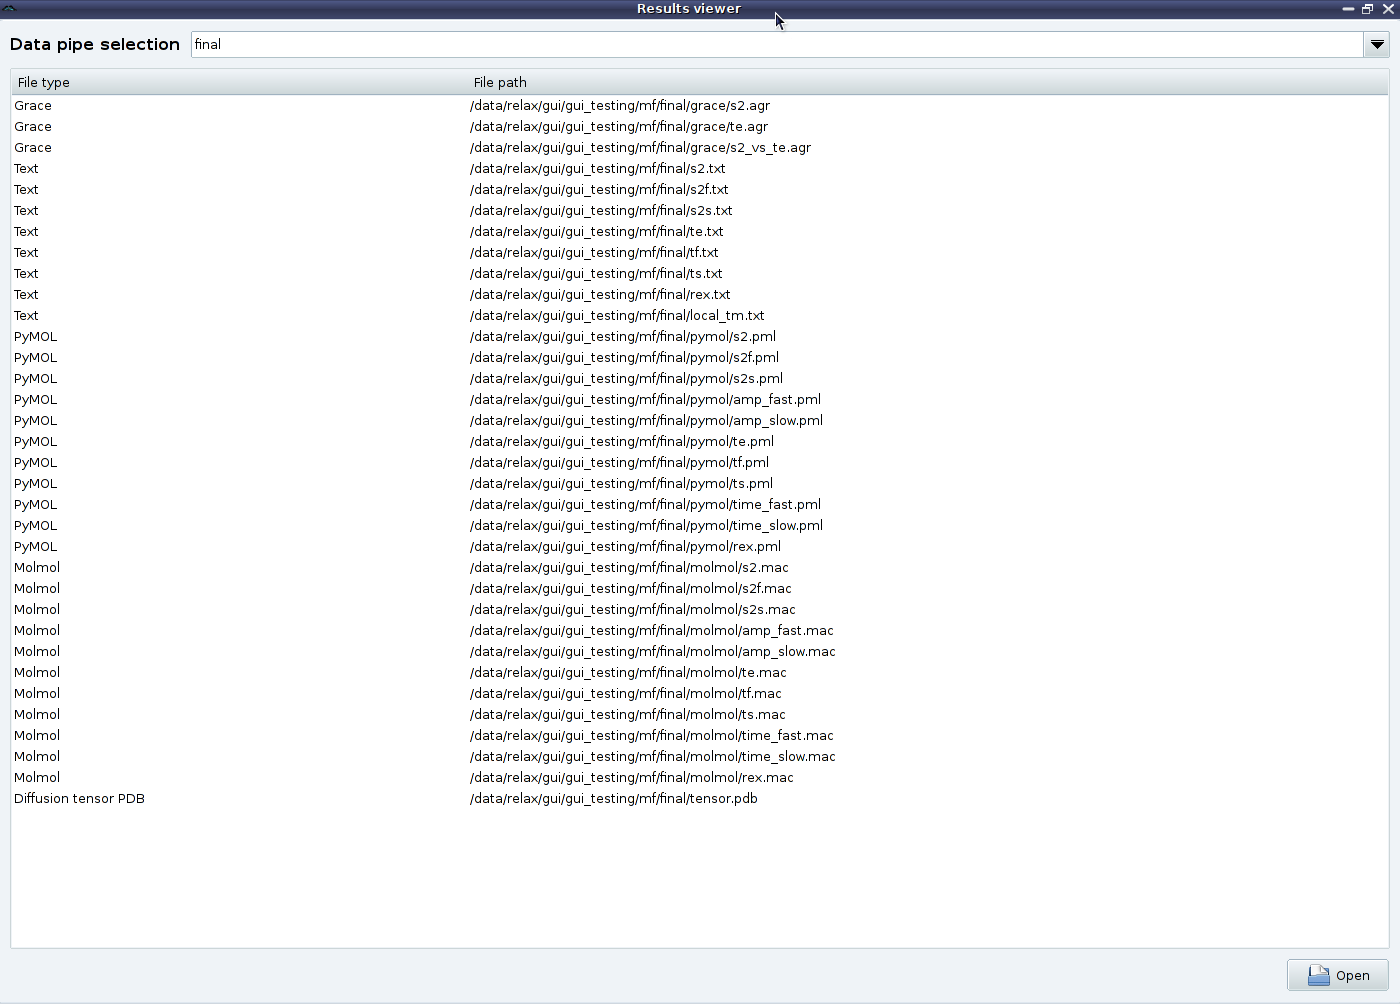
\includegraphics[width=0.9\textwidth, bb=14 14 1065 768]{graphics/screenshots/results_viewer}}
\caption[Results viewer window screenshot]{Screenshot of the relax GUI interface -- the results viewer window.  At the end of one of the automated analyses, a number of results files will be created.  This can include text files containing the results, 2D Grace plots of the results, PyMOL and MOLMOL macros plotting the results onto the structure, diffusion tensor objects for viewing in PyMOL, etc.  This window allows for easy opening of these results files.}\label{fig: screenshot: results viewer}
\end{figure}

% Pipe editor screenshot
\begin{figure}
\centerline{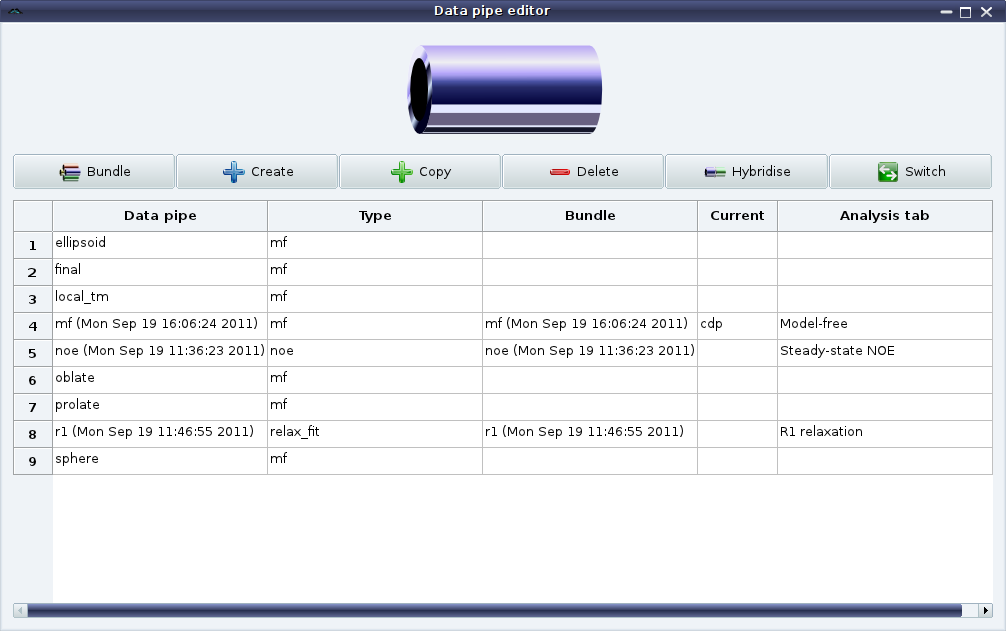
\includegraphics[width=0.9\textwidth, bb=14 14 769 488]{graphics/screenshots/pipe_editor}}
\caption[Pipe editor window screenshot]{Screenshot of the relax GUI interface -- the pipe editor window.  One analysis may consist of one or more data pipes.  And each analysis has its own unique set of data pipes.  This editor allows for the easy manipulation of data pipes for advanced users.}\label{fig: screenshot: pipe editor}
\end{figure}

% Prompt window screenshot
\begin{figure}
\centerline{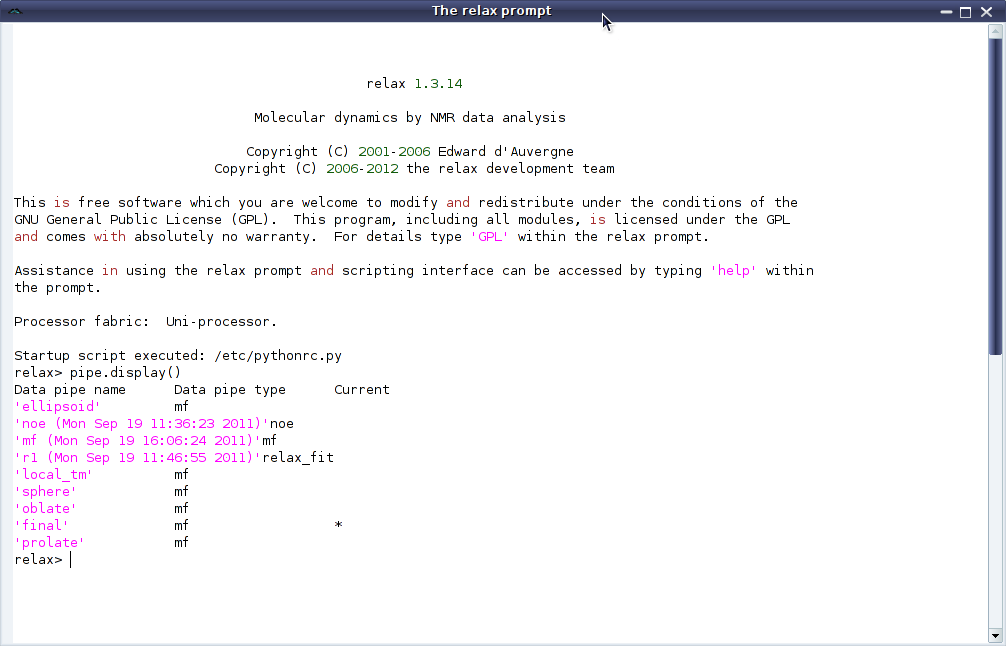
\includegraphics[width=0.8\textwidth, bb=14 14 769 499]{graphics/screenshots/relax_prompt}}
\caption[Prompt window screenshot]{Screenshot of the relax GUI interface -- the prompt window.  This window mimics relax in the prompt user interface mode, and provides the full power of the prompt/script UI modes within the GUI.}\label{fig: screenshot: prompt window}
\end{figure}


\begin{description}
\item[The relax controller]:  This window shows the progress of relax's execution and displays relax's text output for checking if the analysis has been performed correctly and has completed successfully (see Figure~\ref{fig: screenshot: relax controller}).
\item[Spin viewer window]:  This is used to load spins system information into the relax data store and to see the contents of the spin containers (see Figure~\ref{fig: screenshot: spin viewer}).
\item[Results viewer window]:  This presents a list of the results files which can be opened by double clicking for visualisation using a text editor, Grace, PyMOL, MOLMOL, etc (see Figure~\ref{fig: screenshot: results viewer}).
\item[Data pipe editor]:  This window allows for easy manipulation of the data pipes of the relax data store (see Figure~\ref{fig: screenshot: pipe editor}).
\item[The relax prompt]:  This window gives access to the relax prompt (see Figure~\ref{fig: screenshot: prompt window}).
\end{description}



% Access to the internals of relax.
%~~~~~~~~~~~~~~~~~~~~~~~~~~~~~~~~~~

\subsection{Access to the internals of relax}

To enable advanced Python\index{Python} scripting and control, many parts of relax have been designed in an object oriented fashion.
If you would like to play with internals of the program the entirety of relax is accessible by importation.
For example all data is contained within the object called the relax data store which, to be able to access it, needs be imported by typing:

\begin{lstlisting}[numbers=none]
relax> from data_store import Relax_data_store; ds = Relax_data_store()
\end{lstlisting}

The \prompt{ds} object is a dictionary type which contains the multiple data pipes.
All of relax's packages, modules, functions, and classes are also accessible by import statements.
For example to create a rotation matrix from three Euler angles in the z-y-z notation, type:

\begin{lstlisting}[numbers=none]
relax> alpha = 0.1342
relax> beta = 1.0134
relax> gamma = 2.4747
relax> from lib.geometry.rotations import euler_to_R_zyz
relax> from numpy import float64, zeros
relax> R = zeros((3,3), float64)
relax> euler_to_R_zyz(alpha, beta, gamma, R)
relax> print(R)
[[-0.494666415429033 -0.557373756841289 -0.666813041737502]
 [ 0.219125193028791 -0.822460914570202  0.524921131013452]
 [-0.84100492699311   0.113545317776532  0.528978424497956]]
relax>
\end{lstlisting}



% The multi-processor framework.
%%%%%%%%%%%%%%%%%%%%%%%%%%%%%%%%

\section{The multi-processor framework}
\index{multi-processor framework}
\label{sect: multi-processor}



% Introduction.
%~~~~~~~~~~~~~~

\subsection{Introduction to the multi-processor}

Thanks to Gary Thompson's multi-processor framework, relax can be run on multi-core/multi-CPU systems or on clusters to speed up calculations.
As most analyses are relatively quick and would not benefit from the multi-processor framework, only the model-free and frame order analyses have currently been parallelised to run within this framework.
To use the multi-processor framework, the following should be installed:

\begin{description}
\item[\href{http://www.open-mpi.org/}{OpenMPI}\index{MPI!OpenMPI|textbf}:]  This is the most commonly used Message Passing Interface (MPI)\index{MPI} protocol software.
The rest of this manual will assume that this is the implementation in use.
If another implementation is used, please see the specific documentation for that software for how to set up a program to run via MPI.
\item[\href{http://mpi4py.scipy.org/}{mpi4py}\index{MPI!mpi4py|textbf}:]  This dependency is essential for running in MPI mode in relax.
If you would like to use another Python implementation to access the MPI protocol, please consider becoming a relax developer.
\end{description}



% Usage.
%~~~~~~~

\subsection{Usage of the multi-processor}

If you have access to a 256 node cluster and can run calculations on all nodes, assuming that the \file{dauvergne\osus{}protocol.py} automated model-free analysis sample script will be used (after modification for the system under study), relax can be executed by typing:

\example{\$ mpirun -np 257 /usr/local/bin/relax --multi=`mpi4py' --tee log dauvergne\_protocol.py}

Note that the argument \prompt{-np} value is one more than the number of slaves you would like to run.
You should then see the following text in the initial relax printout:

\example{Processor fabric:  MPI 2.1 running via mpi4py with 256 slave processors \& 1 master.  Using Open MPI 1.4.3.}



% Further details.
%~~~~~~~~~~~~~~~~~

\subsection{Further details}

For a full description of the multi-processor framework and how to use it, please see Gary Thompson's official announcement on the \href{https://mail.gna.org/public/relax-devel/2007-05/msg00000.html}{relax-devel mailing list}.



% Usage of the name relax.
%%%%%%%%%%%%%%%%%%%%%%%%%%

\section{Usage of the name relax}

The program relax is so relaxed that the first letter should always be in lower case!
